% Copyright (C) 2018 PUC-Rio/Laboratorio TeleMidia
%
% Permission is granted to copy, distribute and/or modify this document
% under the terms of the GNU Free Documentation License, Version 1.3 or any
% later version published by the Free Software Foundation; with no Invariant
% Sections, with no Front-Cover Texts, and with no Back-Cover Texts. A copy
% of the license is included in the "GNU Free Documentation License" file as
% part of this distribution.

\documentclass[tikz,border=6pt]{standalone}
\usepackage{helvet}
\renewcommand{\familydefault}{\sfdefault}
\usepackage{tikz}
\usetikzlibrary{
  arrows,
  arrows.meta,
  calc,
  math,
  positioning,
  shapes,
}
\tikzset{
node distance=4em,
  x = 2em,
  y = 2em,
  n/.style={
    draw, minimum width=6.5em, minimum height=3em,
    inner sep=0pt, outer sep=0pt, font=\small,
  },
  >=stealth',
  inherit/.style={>={Triangle[open]}},
  has/.tip={Diamond[open]},
}
\begin{document}
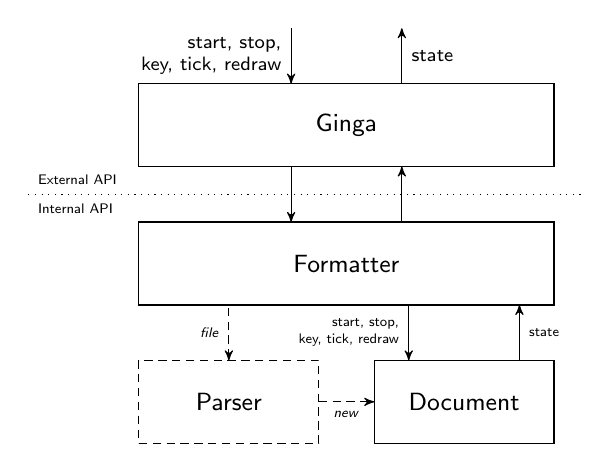
\begin{tikzpicture}[
  node distance=2em,
  b/.style={font=\scriptsize},
  c/.style={font=\tiny},]
  %%
  \node[n, minimum width=15em](Ginga){Ginga};
  \node[n, below=of Ginga,minimum width=15em](Fmt){Formatter};
  \node[n, below=of Fmt.south west, anchor=north west,
  densely dashed]
  (Parser){Parser};
  \node[n,below=of Fmt.south east, anchor=north east]
  (Doc){Document};
  %%
  \draw[->]($(Ginga.north)+(-1,1)$)
  -- node[b,left,text width=6em, align=right]
  {start, stop,\\key, tick, redraw} ($(Ginga.north)+(-1,0)$);
  %%
  \draw[<-]($(Ginga.north)+(1,1)$)
  -- node[b,right,text width=6em] {state} ($(Ginga.north)+(1,0)$);
  %%
  \draw[dotted]
  ($($(Ginga.south west)+(-4,0)$)!.5!(Fmt.north west)$)
  node[c,above,anchor=south west] {External API}
  node[c,below,anchor=north west] {Internal API}
  -- ($(Ginga.south east)!.5!($(Fmt.north east)+(1,0)$)$);
  %%
  \draw[->]($(Fmt.north)+(-1,1)$) -- ($(Fmt.north)+(-1,0)$);
  \draw[<-]($(Fmt.north)+(1,1)$) -- ($(Fmt.north)+(1,0)$);
  %%
  \draw[<-,densely dashed](Parser.north)
  -- node[c,left] {\emph{file}} ($(Parser.north)+(0,1)$);
  \draw[->,densely dashed](Parser.east)
  -- node[c,below] {\emph{new}} (Doc.west);
  %%
  \draw[->]($(Doc.north)+(-1,1)$)
  -- node[c,left,text width=4em, align=right]
  {start, stop,\\key, tick, redraw} ($(Doc.north)+(-1,0)$);
  \draw[<-]($(Doc.north)+(1,1)$)
  -- node[c,right] {state} ($(Doc.north)+(1,0)$);
\end{tikzpicture}

\cleardoublepage
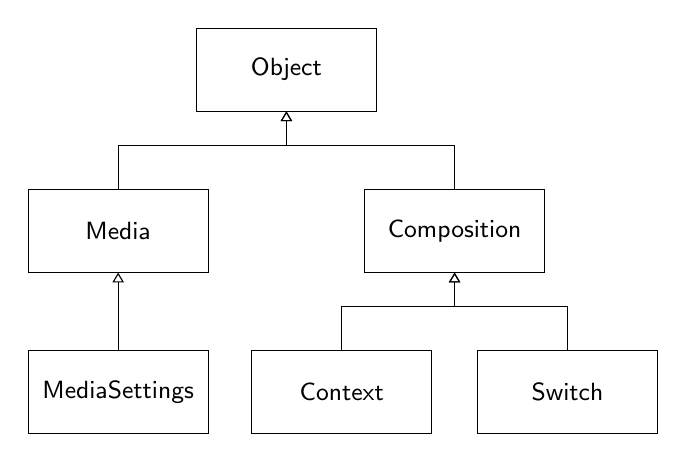
\begin{tikzpicture}
  \node[n](Obj){Object};
  \node[n, below left=of Obj.south](Med){Media};
  \node[n, below right=of Obj.south](Comp){Composition};
  %%
  \node[n, below left=of Comp.south, xshift=2em](Ctx){Context};
  \node[n, below right=of Comp.south, xshift=-2em](Swtc){Switch};
  %%
  \node[n](Set) at (Ctx-|Med){MediaSettings};
  %%
  \draw[inherit,->](Med.north) -- ++(0,.8) -| (Obj.south);
  \draw[inherit,->](Comp.north) -- ++(0,.8) -| (Obj.south);
  %%
  \draw[inherit,->](Ctx.north) -- ++(0,.8) -| (Comp.south);
  \draw[inherit,->](Swtc.north) -- ++(0,.8) -| (Comp.south);
  %%
  \draw[inherit,->](Set.north) -- (Med.south);
\end{tikzpicture}

\cleardoublepage
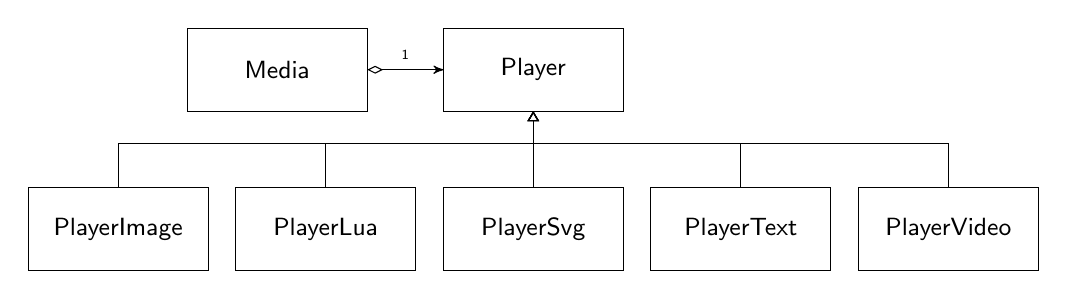
\begin{tikzpicture}[node distance=2.75em]
  \node[n](Med){Media};
  \node[n, right=of Med](Play){Player};
  \node[n, below=of Play](C){PlayerSvg};
  \begin{scope}[node distance=1em]
    \node[n, left=of C](B){PlayerLua};
    \node[n, left=of B](A){PlayerImage};
    \node[n, right=of C](D){PlayerText};
    \node[n, right=of D](E){PlayerVideo};
  \end{scope}
  \draw[inherit,->](A.north) -- ++(0,.8) -| (Play.south);
  \draw[inherit,->](B.north) -- ++(0,.8) -| (Play.south);
  \draw[inherit,->](C.north) -- (Play.south);
  \draw[inherit,->](D.north) -- ++(0,.8) -| (Play.south);
  \draw[inherit,->](E.north) -- ++(0,.8) -| (Play.south);
  %%
  \draw[{has}->](Med.east) -- node[font=\tiny,above]{1} (Play.west);
\end{tikzpicture}
\end{document}
